\begin{center}
    \Large{\textbf{Відповіді на контрольні питання}}    
\end{center}

\vspace{1mm}

\begin{enumerate}
    \item Що таке дійсне, уявне зображення?  
    \bigbreak
    Дійсне зображення - зображення утворене перетином безпосередньо самих
    заломлених променів.

    Уявне зображення - зображення утворене перетином уявних продовжень
    заломлених променів.

    \item За яких умов створюється дійсне зображення для збиральної лінзи?
    \bigbreak
    
    Дійсне зображення для збиральної лінзи створюється за умови
    розташування предмета на відстані більшу за фокусну.

    \item За яких умов створюється уявне зображення у схемах зі збиральною лінзою?
    \bigbreak
    Якщо предмет розташований на відстані, яка менша фокусної відстані, то
    утворюється уявне зображення.

    \item За яких умов не бачимо зображення?
    \bigbreak

    Ми не бачимо зображення(для збиральної лінзи), коли
    предмет розташований на фокусній відстані від лінзи.

    \item Хід променів для кожного вищевказаного випадку?
    \bigbreak

    Хід променів при створенні дійсного зображення.

    \begin{figure}[h!]
        \hfill
        \begin{minipage}[h]{0.3\linewidth}
            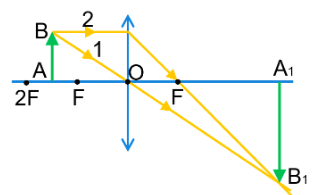
\includegraphics[height = 3cm]{assets/F2F.png}
            \caption{$F < g < 2F$}
        \end{minipage}        
        \begin{minipage}[h]{0.32\linewidth}
            \vfill
            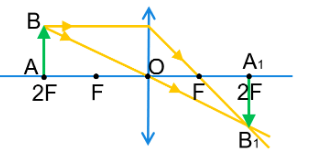
\includegraphics[height = 2.7cm]{assets/2F.png}
            \vspace{0.1cm}
            \caption{$g = 2F$}
        \end{minipage}
        \begin{minipage}[h]{0.32\linewidth}
            \vfill
            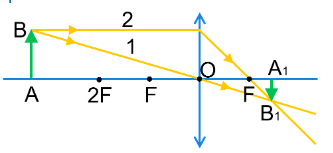
\includegraphics[height = 2.7cm]{assets/G2F.png}
            \vspace{0.1cm}
            \caption{$g > 2F$}
        \end{minipage}
    \end{figure}

    Хід променів при створенні увного $g < F$ зображення та 
    для варіанту, коли ми не бачимо зображення$g = F$.

    \begin{figure}[ht!]        
        \begin{minipage}[h]{0.6\linewidth}
            \hspace{2cm}
            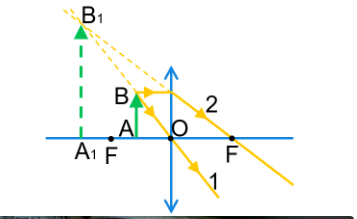
\includegraphics[height = 3.3cm, trim={0, 2mm, 0, 0},clip]{assets/LessF.png}
            \caption{$g < F$ - уявне зображення}
        \end{minipage} 
        \hfill       
        \begin{minipage}[h]{0.45\linewidth}        
            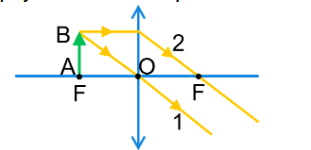
\includegraphics[height = 2.9cm]{assets/F.png}
            \vspace{0.5cm}
            \caption{$g = F$ - немає зображення}
        \end{minipage}
    \end{figure}

    
    \bigbreak
    \bigbreak
    \bigbreak
    \bigbreak
    \bigbreak
    \item Що таке сферична аберація?
    \bigbreak
    Похибка, пов'язана із сферичністю заломлюючих поверхонь.
    Якщо із джерела виходить пучок світла, який утворює з
    головною оптичною віссю великий кут, то промені, які утворюють різні 
    кути, перетинають оптичну вісь не в одній, а в різних точках.
    Промені, більш віддалені від центра лінзи, більше заломлюються 
    і перетинають головну оптичну вісь на порівняно близьких відстанях від центра 
    лінзи. Якщо екран, розташований перпендикулярно до головної оптичної осі,
    то замість точкового зображення буде розпливчаста пляма.

    \item Що таке хроматична аберація?
    \bigbreak
    Спотворення зображення, яке характеризується 
    чергуванням кольорів в залежності від положення екрана.
    Залежність показника залом­лення речовини лінзи від довжини 
    світлової хвилі(дис­персія) призводить до того, що фокуси для 
    різних кольорів зміщені один відносно одного. У результаті 
    зображення білої плями виходить кольоровим.

    \item В чому полягає різниця між тонкою і звичайною лінзою?
    \bigbreak

    Лінзою називається прозоре тіло, обмежене двома сферичними поверхнями.
    Якщо товщина самої лінзи мала в порівнянні з радіусами кривизни 
    сферичних поверхонь, то лінзу називають тонкою. Тобто тонкі лінзи - це тільки
    підмножина усіх лінз.

\end{enumerate}